%%%%%%%%%%%%%%%%%%%%%%%%%%%%%%%%%%%%%%%%%%%%%%%%%%%%%%%%%%%%%%%%%%%%%%%%
%                                                                      %
% LaTeX, FIIW thesis template                                          %
%                                                                      %
%%%%%%%%%%%%%%%%%%%%%%%%%%%%%%%%%%%%%%%%%%%%%%%%%%%%%%%%%%%%%%%%%%%%%%%%
\documentclass[11pt,a4paper,twoside]{book}
% If you want to print your thesis double sided, you can use the settings below
%\documentclass[11pt,a4paper,twoside,openright]{report}

%%% Load the FIIW template
%%% You should specify your campus : groept, denayer, gent, geel and brugge are implemented
%%% You can hide parts of the preface by specifying some option:
%%% e.g. : noacknowledgements, noabstract, noextendedabstract, nolistoffigures, nolistoftables, nolistofsymbols
\usepackage[groept]{fiiw}


%%% Load some other basic packages
\usepackage[dutch,english]{babel}
\usepackage[latin1]{inputenc}           % needed if you have special characters in your text
%\usepackage[utf8]{inputenc}            % if your text is encoded in utf8 (and not latin1) use this package

\usepackage{natbib}						% used for cites from the bib file in your text
\usepackage{listings}             		% used for displaying source code (java, c, matlab,...)
\usepackage{verbatim}					% used for inline formatting of source code, terminal commands, ...
\usepackage{hyperref}					% include hyperlinks in the resulting PDF
\usepackage{url}						% add url's with \url{http://}
\usepackage[final]{pdfpages}            % include pdf's e.g.: a paper or a poster
%\usepackage[times]{quotchap}           % if you want realy fancy chapter titles...
\usepackage{float}                      % adds [H] to figure env. Puts a figure where you want it e.g. \begin{figure}[H]
\usepackage{longtable}					% used for tables that strech over muliple pages

% generate lorum ipsim text in template
\usepackage{lipsum}

%%% configure layout for source code listings
%\definecolor{keyword}{rgb}{0.3,0.3,0.3}
\lstset{
	language = Java,
	basicstyle=\scriptsize\ttfamily,
	numbers=left,
	numberstyle=\tiny,
	tabsize=2,
	showspaces=false, 
	frame=single,
	breaklines=true,
%	keywordstyle=\bfseries\color{keyword},
%	stringstyle=\color{string},
	extendedchars=true,
	xleftmargin=0.3\linewidth,
	xrightmargin=0.1\linewidth
}

%%% abstract, acknowledgements and list of figures are located in an other file
%%% list the filenames where you created them. If you omit one of these the page
%%% is not displayed
\acknowledgementsfile{chapters/acknowledgements}			%.tex file with acknowledgements
\abstractfile{chapters/abstract}					%.tex file with abstract
\extendedabstractfile{chapters/abstract-extended}	%.tex file with extended abstract
\listofsymbolsfile{chapters/symbols}				%.tex file with list of symbols
\renewcommand{\appendixname}{List of appendices}
%%% information about you, your thesis, promotor, ...
\program{Electronics Engineering}
\title{OpenProject Plugin Development using Ruby on Rails}
%\subtitle{Thesis Subtitle (optional)}
\firstnameA{Han}
\lastnameA{Li}
%\firstnameB{Firstname2}
%\lastnameB{Lastname2}
\academicyear{2017 - 2018}
%\embargo{12-12-2012}

\promotor{Jeroen Van Aken}
\copromotor{Jeroen Van Aken\newline(Jeroen Van Aken)}
\begin{document}
	%%% select the overall language of the text
	%\selectlanguage{dutch}
	\selectlanguage{english}

	\preface
	\chapter{Introduction}

The purpose of the Introduction should be to supply sufficient background information\footnote{state briefly and clearly your purpose for writing the paper} to the reader to situate, understand and value the results of the present study.\par

\section{Requirements analysis}

The Requirements analysis (or similar title) typically lists requirements (e.g. use cases and/or use case diagrams), scenarios of use, functional and non-functional requirements coming from other (non-) engineering departments.\par

\lipsum[1-7]
 




	\chapter{Design/Materials}

Requirements might be followed by a "Design" chapter, or an Architecture chapter, or a "Systems overview", or a similar title that describes you're the high-level designs. If necessary you can still split this up in several chapters. While not mandatory, if you did undertake efforts to evaluate the quality of your designs or high-level architectures, it is wise to include this information as well. Obviously, students should always try to justify the choices they made (technologies, components, interfaces, etc.)\par

With design choices always state your references \citep{Castleman98,Granlund95} or say that \citet{Holmes95} did good work on some subject.

\section{System Design}
At a system level, this part of the paper could contain:
\begin{itemize}
\item Mechanic components
\item User Interface components
\item Hardware and/or software partitioning
\item Hardware schemas of the main building blocks and interfaces between those building blocks
\item Software components and main interfaces between those components
\end{itemize}

Again, figures and schemas can certainly augment the legibility of the paper, however ensure to also describe the design or architecture in words.\par

\section{Component level Design}
At the component level, a detailed design of the different blocks or modules should be given (e.g. flow diagrams, class/sequence/state diagrams, etc.)\par


	\chapter{Development/Implementation/Methods}
 
Students should mention implementation environment (tools, OS) and other relevant information (code, special sensors, etc.). Obviously, students should not provide every action or every line of code but only that information that is relevant to the reader in order to understand the specifics of the implementation.\par

\begin{figure}
	\centering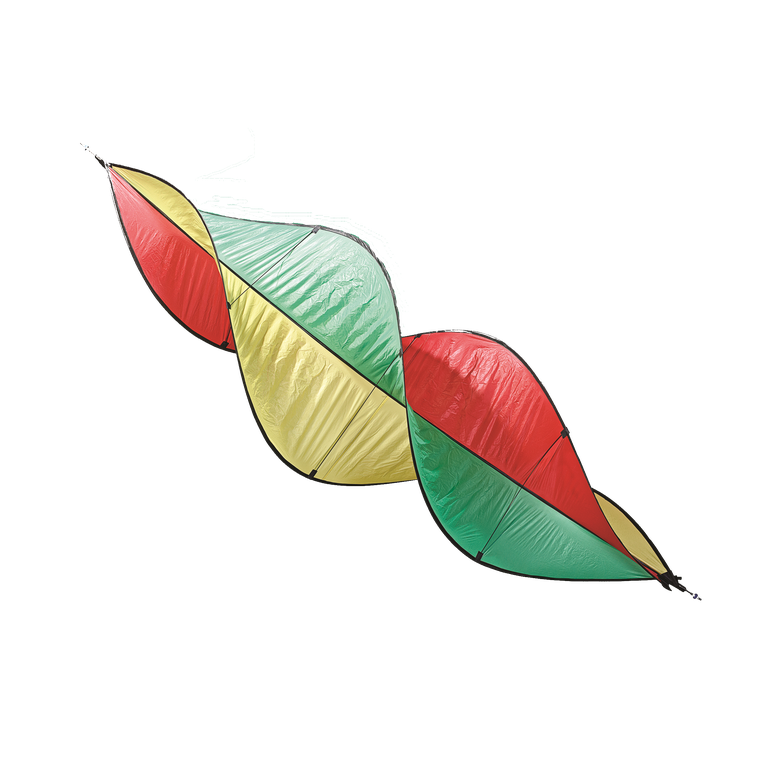
\includegraphics[width=7cm]{./images/fiiw}
	\caption{The FIIW logo}
\end{figure}

\lipsum[1]

\lipsum[1]
 
\section{System Setup}
\lipsum[1]

\section{Mechanical Construction}
\lipsum[1]

\section{Software Implemenation}
\begin{figure}
	\lstset{language=Java}
	\lstinputlisting{listings/example.java}
	\caption{Some example Java code in a listing}
\end{figure}
\lipsum[1]
	\chapter{Evaluation/Validation/Results}

This evaluation could be an evaluation with users, but it could also be stress testing, accuracy tests, bug tests, strength tests, etc. After this evaluation chapter, you should also add the Discussion chapter as described below.

\begin{table}[h]\centering
	\begin{tabular}{|l|c|c|}
		\hline
		Day & Min Temp & Max Temp \\ \hline
		Monday & 11C & 22C \\ \hline
		Tuesday & 9C & 19C \\ \hline
		Wednesday & 10C & 21C \\
		\hline
	\end{tabular}
	\caption{Day to day measurements}
	\label{tab:truthTables}  
\end{table}
	\chapter{Discussion}
 
The Discussion is harder to define than the other sections. It is usually the hardest section to write. 

Firstly, reflect on the problem or research question that you presented in the Introduction. 'frame' your results with respect to the research question or the problem you are trying to solve. Was your approach to solving the problem a good one? Was it the best? Would you recommend it to future engineers?

A discussion is also a place for reflection and for advice/warnings to other researchers. Here you can write how the research could still be improved and what future researchers should focus on. Point out any exceptions or any lack of correlation and define unsettled points. Never take the high-risk alternative of trying to cover up or fudge data that do not quite fit. If this is a particularly long section, it could also become a new section called "Future work".

	\chapter{Conclusion}
 
A separate "Conclusions" section should be incorporated after the Discussion. A conclusion is a summary of your work, a reader that only reads the conclusion should still get the main contribution of your work. A good model of a conclusion is to think of it as an extended abstract in which you can put more stress on the results and why your work is important. Remember that it should be possible for a reader to read only the conclusion and not the rest of your paper, s/he should still get the main points of your work. You definitely need to end your paper with highlighting the significance of your work. Do not make the mistake of providing new information in a conclusion.
	
	%%% Bibliography: references. included from bibliography.bib
	%%% Only referenced items are displayed in the final document
	%\nocite{*}			% if you want to display all items in your bibliografy uncomment this
	\bibliographystyle{apalike}
	\bibliography{bibliography}
	
	
	%%% appendices
    \appendix
    \appendixpage
	\chapter{Some extra info }

\lipsum[5-10]
	
	%%% Apendix from othe pdf
	%\chapter{Poster}
	%\includepdf{poster.pdf}

	\backcover
\end{document}
